%LTeX: language=es-AR
\documentclass[
11pt, % The default document font size, options: 10pt, 11pt, 12pt
]{charter} 
% Paquete para diagramas de Gantt en LaTeX
\usepackage{pgfgantt}
\usepackage{graphicx}
\usepackage{pdflscape}
\usepackage[spanish]{babel}


% El títulos de la memoria, se usa en la carátula y se puede usar el cualquier lugar del documento con el comando \ttitle
\titulo{Predicción de riesgos financieros y estimaciones presupuestarias en construcción inmobiliaria con modelos de aprendizaje automático} 

% Nombre del posgrado, se usa en la carátula y se puede usar el cualquier lugar del documento con el comando \degreename
%\posgrado{Carrera de Especialización en Sistemas Embebidos} 
%\posgrado{Carrera de Especialización en Internet de las Cosas} 
\posgrado{Carrera de Especialización en Inteligencia Artificial}
%\posgrado{Maestría en Sistemas Embebidos} 
%\posgrado{Maestría en Internet de las cosas}

% Tu nombre, se puede usar el cualquier lugar del documento con el comando \authorname
% IMPORTANTE: no omitir titulaciones ni tildación en los nombres, también se recomienda escribir los nombres completos (tal cual los tienen en su documento)
\autor{Ing. Danilo Simón Reitano Andrades}

% El nombre del director y co-director, se puede usar el cualquier lugar del documento con el comando \supname y \cosupname y \pertesupname y \pertecosupname
% \director{Dr. Ing. Hernán Garrido}
% \pertenenciaDirector{Prof. Titular – FING, UNCUYO}
\director{A definir}
\pertenenciaDirector{A definir}

% Nombre del cliente, quien va a aprobar los resultados del proyecto, se puede usar con el comando \clientename y \empclientename
\cliente{Martin Brambati}
\empresaCliente{Built Technologies}
 
\fechaINICIO{29 de abril de 2025}		%Fecha de inicio de la cursada de GdP \fechaInicioName
\fechaFINALPlan{17 de junio de 2025} 	%Fecha de final de cursada de GdP
\fechaFINALTrabajo{30 de noviembre de 2024}	%Fecha de defensa pública del trabajo final


\begin{document}

\maketitle
\thispagestyle{empty}
\pagebreak


\thispagestyle{empty}
{\setlength{\parskip}{0pt}
\tableofcontents{}
}
\pagebreak


\section*{Registros de cambios}
\label{sec:registro}


\begin{table}[ht]
\label{tab:registro}
\centering
\begin{tabularx}{\linewidth}{@{}|c|X|c|@{}}
\hline
\rowcolor[HTML]{C0C0C0} 
Revisión & \multicolumn{1}{c|}{\cellcolor[HTML]{C0C0C0}Detalles de los cambios realizados} & Fecha      \\ \hline
0      & Creación del documento                                 &\fechaInicioName \\ \hline
1      & Se completa hasta el punto 5 inclusive                & 12 de mayo de 2025 \\ \hline
2      & Se completa hasta el punto 9 inclusive               & 19 de mayo de 2025 \\ \hline
%		  Se puede agregar algo más \newline
%		  En distintas líneas \newline
%		  Así                                                    & {día} de {mes} de 202X \\ \hline
%3      & Se completa hasta el punto 12 inclusive                & {día} de {mes} de 202X \\ \hline
%4      & Se completa el plan	                                 & {día} de {mes} de 202X \\ \hline

% Si hay más correcciones pasada la versión 4 también se deben especificar acá

\end{tabularx}
\end{table}

\pagebreak



\section*{Acta de constitución del proyecto}
\label{sec:acta}

\begin{flushright}
Mendoza, \fechaInicioName
\end{flushright}

\vspace{2cm}

Por medio de la presente se acuerda con el \authorname\hspace{1px} que su Trabajo Final de la \degreename\hspace{1px} se titulará ``\ttitle'' y consistirá en el desarrollo un modelo de predicción de préstamos y presupuestos de construcción. El trabajo tendrá un presupuesto preliminar estimado de 600 horas y un costo estimado de \$ 1500, con fecha de inicio el \fechaInicioName\hspace{1px} y fecha de presentación pública a definir.

Se adjunta a esta acta la planificación inicial.

\vfill

% Esta parte se construye sola con la información que hayan cargado en el preámbulo del documento y no debe modificarla
\begin{table}[ht]
\centering
\begin{tabular}{ccc}
\begin{tabular}[c]{@{}c@{}}Dr. Ing. Ariel Lutenberg \\ Director posgrado FIUBA\end{tabular} & \hspace{2cm} & \begin{tabular}[c]{@{}c@{}}\clientename \\ \empclientename \end{tabular} \vspace{2.5cm} \\ 
\multicolumn{3}{c}{\begin{tabular}[c]{@{}c@{}} \supname \\ Director del Trabajo Final\end{tabular}} \vspace{2.5cm} \\
\end{tabular}
\end{table}




\section{1. Descripción técnica-conceptual del proyecto a realizar}
\label{sec:descripcion}

\subsection*{Introducción, contexto y propuesta de solución}

El presente trabajo surge a partir de una necesidad concreta de Built Technologies, empresa con sede en Nashville, Tennessee, Estados Unidos. Dicha necesidad de responder preguntas sobre los presupuestos de sus clientes fue identificada por el autor del documento, Danilo Reitano. Dicha empresa desarrolla una plataforma SaaS líder en la gestión de préstamos para la construcción. Trabaja con múltiples entidades bancarias y financieras que otorgan financiamiento a personas que planean construír su casa, desarrolladores y contratistas para la ejecución de proyectos residenciales y comerciales. La plataforma permite monitorear el uso del préstamo, la ejecución del presupuesto y los avances del proyecto de forma integrada.

Uno de los principales desafíos operativos que enfrenta la empresa, y en general el sector de préstamos para construcción, es la dificultad para validar en etapas tempranas si el importe del préstamo solicitado por el cliente será suficiente para cubrir los costos del proyecto. Actualmente, esta validación se realiza mediante revisiones manuales de los presupuestos enviados, que suelen estar desagregados en múltiples partidas (ej. cimentación, materiales, permisos, mano de obra, pisos, techos, terminaciones, etc.). Este proceso es altamente dependiente del criterio del analista y de las experiencias pasadas, sin una herramienta sistemática que permita predecir desvíos, subestimaciones o riesgos de insuficiencia presupuestaria. A menudo, estas deficiencias recién se manifiestan cuando el proyecto ya está en ejecución, mientras se generan sobrecostos, atrasos, renegociaciones contractuales o incluso abandono de obra.

En este contexto, la propuesta de esta tesis es el desarrollo de un sistema predictivo basado en modelos de aprendizaje automático que permita asistir de manera inteligente a los analistas de crédito en dos aspectos clave:

\begin{enumerate}
    \item Estimar, a partir de la información disponible al momento de analizar el préstamo, si el importe solicitado será suficiente para cubrir el presupuesto completo del proyecto.
    \item Predecir los costos esperados para cada una de las partidas presupuestarias del proyecto (por ejemplo: excavación, estructura, instalaciones eléctricas, techado, acabados). Se deberá tener en cuenta características del proyecto como su ubicación, tipo, proveedor, constructor, superficie y otros factores históricos.
\end{enumerate}

Este doble enfoque con distintas capas de análisis permitirá no solo detectar situaciones de riesgo financiero de manera temprana, sino también ofrecer recomendaciones concretas sobre los costos esperados. Todo esto en función de los datos históricos, ajustados al contexto de cada proyecto.

\subsection*{Contexto y condiciones particulares del proyecto}

Este proyecto se desarrollará en estrecha colaboración con el equipo de datos de Built Technologies. Se cuenta con acceso autorizado a un dataset anonimizado que incluye información detallada de más de 10 años de historial de proyectos, con datos por rubro presupuestario, tipo de préstamo, ubicación, resultados de ejecución y características del contratista y del proveedor. Por cuestiones de privacidad y cumplimiento normativo (SOC 2 y GDPR), los datos no contienen información sensible de clientes, y el trabajo se limita exclusivamente a información estructurada, sin el uso de documentos escaneados o imágenes.

\subsection*{Estado del arte y diferenciación de la solución}

En términos generales, existen diversas aplicaciones de modelos de machine learning en el ámbito financiero, particularmente en la evaluación de crédito, detección de fraude y puntuación de clientes. Sin embargo, el uso de aprendizaje automático para prever costos de construcción y validar la suficiencia de préstamos basándonos en presupuestos históricos es aún una línea de investigación y desarrollo incipiente.

La mayoría de las soluciones actuales en el sector se apoyan en heurísticas basadas en precios unitarios, bases de datos estáticas por región o \textit{benchmarking} manual entre proyectos. Esto tiene limitaciones evidentes: no contempla el contexto completo del proyecto ni aprende de los patrones reales de ejecución observados en los últimos años. Además, a medida que los proyectos modernos incrementaron en escala y complejidad, los métodos convencionales resultan insuficientes para capturar todas las variables que afectan los costos.

La regresión multivariada ha sido un enfoque base para estimar costos de construcción. Estos modelos asumen relaciones lineales entre los factores (como tamaño de la obra, calidad de los materiales, etc.) y el costo total. En escenarios relativamente simples, las regresiones pueden brindar estimaciones razonables: típicamente logran una precisión del orden de 75 \%-80 \%. No obstante, en la mayoría de proyectos existen relaciones no lineales y dependencias complejas entre variables (economías de escala, influencias del mercado, interacciones entre diseño y método constructivo) que limitan la capacidad predictiva.

También se ha explorado la utilización de otro tipo de modelos como \textit{Random Forest} y \textit{XGBoost}. Estos enfoques han mostrado mejoras significativas en precisión frente a métodos tradicionales. Por ejemplo, un estudio recopiló datos de 95 proyectos de edificios y implementó un modelo de \textit{Random Forest} para predecir riesgos de sobrecostos. Otro ejemplo relevante es un trabajo que utiliza \textit{XGBoost} para seleccionar las variables más influyentes y estimar el costo de proyectos de edificación.

En otros casos, se ha explorado la posibilidad de utilizar modelos de \textit{deep learning} para estimación de costos en el desarrollo de proyectos. Algunas investigaciones han resultado en precisiones del 85 \%-90 \%, superior a la obtenida por modelos más simples. Esto se traduce en menores errores de predicción para proyectos complejos, aunque a costa de una mayor demanda de datos y capacidad computacional.

Al leer los resultados de dichos proyectos, se puede apreciar que las variables de mayor influencia son la escala del proyecto (metros cuadrados construídos, número de plantas), funcionalidad (edificio residencial, comercial, salud, etc.), así como especificaciones técnicas principales (tipo de climatización, sistema estructural, acaados exteriores e interiores, presencia de elementos especiales como ascensores, etc.), ubicación geográfica, año o época de construcción y tipo de contrato, entre otros.


La solución propuesta se diferencia en que:
\begin{itemize}
    \item Utiliza modelos de aprendizaje supervisado entrenados sobre datos reales de ejecución y financiamiento, con ajuste de las predicciones al comportamiento histórico.
    \item Integra múltiples variables categóricas y numéricas, como ubicación geográfica, superficie construida, tipo de contratista y composición del presupuesto, con una predicción contextualizada.
    \item Utiliza un volumen de datos mayor a los proyectos realizados hasta el momento.
    \item Incorpora técnicas de explicabilidad como SHAP (Shapley Additive Explanations) para interpretar por qué el modelo predice insuficiencia o sobrecosto, con adopción por parte de analistas humanos.
    \item Ofrece tanto una salida binaria (¿es suficiente el préstamo?) como una salida regresiva multirrubro (estimación de costos por partida).
\end{itemize}

\subsection*{Propuesta de valor e impacto esperado}

La implementación de este sistema generará múltiples beneficios para Built Technologies y sus socios financieros:

\begin{itemize}
    \item Reducir el porcentaje de proyectos con préstamos insuficientes y así lograr evitar renegociaciones y sobrecostos.
    \item Mejorar la eficiencia del análisis crediticio, donde los analistas cuentan con una herramienta predictiva basada en datos.
    \item Aumentar la satisfacción del cliente final, sin interrupciones en la ejecución del proyecto por errores de estimación.
    \item Detectar patrones de subestimación crónica en ciertos rubros o regiones, lo que podría informar futuras políticas de originación de préstamos.
\end{itemize}

El sistema se implementará inicialmente como un prototipo funcional con salida en formato tabular y visual, para luego ser integrado en el flujo de trabajo de análisis crediticio mediante una API o módulo dentro de la plataforma existente.

\subsection*{Descripción funcional de la solución}

La solución se compone de los siguientes bloques funcionales:

\begin{itemize}
    \item \textbf{Módulo de extracción de datos}: identificación, scrapping y unificación de datos.
    \item \textbf{Módulo de procesamiento de datos}: limpieza, transformación y validación de los datos históricos estructurados.
    \item \textbf{Módulo de entrenamiento}: entrenamiento de dos modelos: uno de clasificación binaria (suficiencia del préstamo) y otro de regresión multirrubro (predicción de costos por partida).
    \item \textbf{Módulo de inferencia}: dado un nuevo proyecto con sus características, el sistema entrega predicciones de suficiencia y una tabla con los valores esperados por rubro presupuestario.
    \item \textbf{Módulo de visualización}: presenta los resultados a través de gráficos, tablas y explicaciones interpretables para el uso por parte del equipo financiero.
\end{itemize}

En la figura \ref{fig:diagBloques} se presenta el diagrama en bloques del sistema. Se observa el flujo de datos desde la base histórica, las etapas de preprocesamiento, entrenamiento e inferencia, hasta la visualización de resultados por parte del analista financiero.

\begin{figure}[htpb]
\centering 
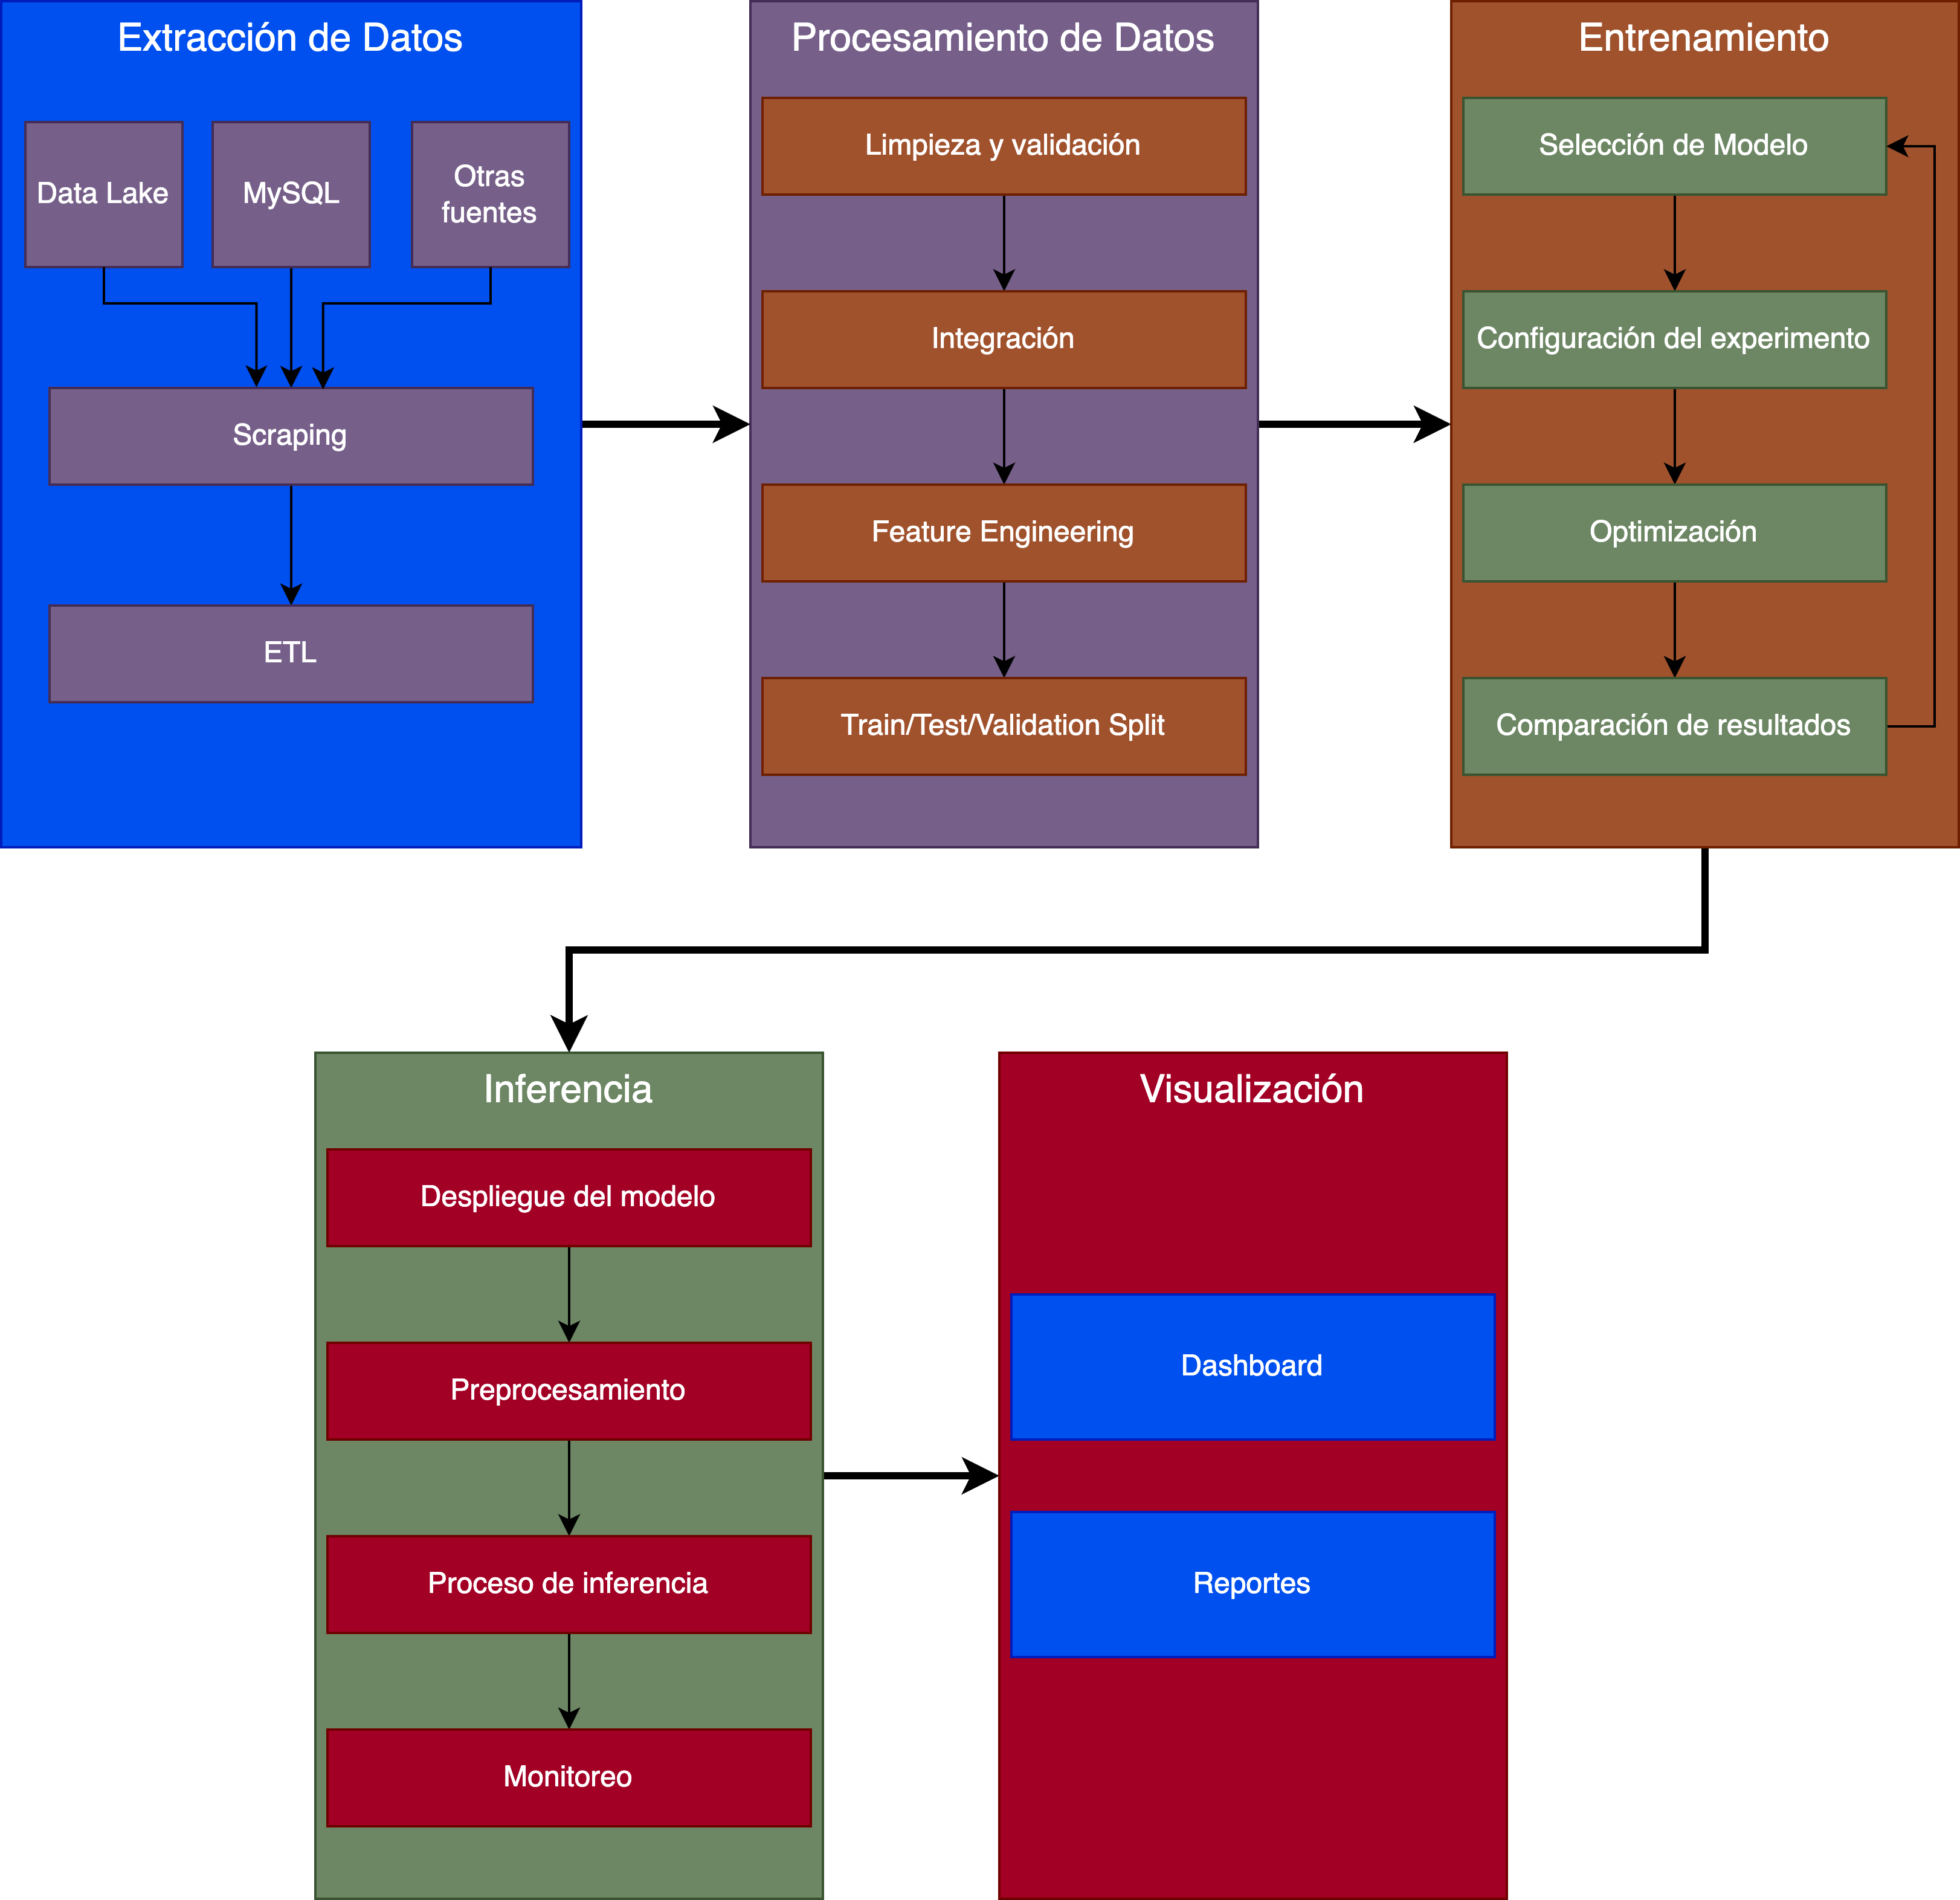
\includegraphics[width=1\textwidth]{./Figuras/bloques.png}
\caption{Diagrama en bloques del sistema.}
\label{fig:diagBloques}
\end{figure}

\section{2. Identificación y análisis de los interesados}
\label{sec:interesados}

\begin{table}[ht]
%\caption{Identificación de los interesados}
%\label{tab:interesados}
\begin{tabularx}{\linewidth}{@{}|l|X|X|l|@{}}
\hline
\rowcolor[HTML]{C0C0C0} 
Rol           & Nombre y Apellido & Organización         & Puesto \\ \hline
Cliente       & \clientename      &\empclientename       & Engineering Manager \\ \hline
Responsable   & \authorname       & FIUBA        	       & Alumno \\ \hline
Colaboradores & Thomas Schlegel   &\empclientename       & Distinguished Engineer	\\ \hline
Orientador    & \supname	        & \pertesupname 	     & Director del Trabajo Final \\ \hline
Opositores    & -                 & Procore Technologies & - \\ \hline
Usuario final & -                 & Clientes de Built 	 & - \\ \hline
\end{tabularx}
\end{table}

\begin{itemize}
	\item Orientador: a definir.
	\item Cliente: Martin Brambati posee una amplia trayectoria como mánager y director de ingeniería. Su experiencia será de gran valor para el desarrollo del proyecto.
	\item Colaboradores: Thomas Schlegel cuenta con más de 8 años de experiencia a cargo del área de datos en Built Technologies, lo que será de gran ayuda para la comprensión del conjunto de datos.
	\item Opositores: Procore Technologies proporciona una plataforma unificada de gestión financiera de proyectos de construcción. La empresa incorporó anteriormente herramientas de inteligencia artificial, por la que tendría intenciones de que este proyecto no llegue a concluirse.
\end{itemize}

\section{3. Propósito del proyecto}
\label{sec:proposito}

Desarrollar una solución basada en modelos de aprendizaje automático que permita asistir a los analistas financieros de Built Technologies en la evaluación de la suficiencia de préstamos otorgados para proyectos de construcción. Dicha solución deberá orientar en la estimación detallada de los costos asociados a cada una de las partidas presupuestarias. La solución busca anticipar riesgos de subfinanciamiento y sobrecostos mediante el análisis de datos históricos anonimizados. Esto produce decisiones más informadas, eficientes y escalables dentro del flujo de originación de créditos.

\section{4. Alcance del proyecto}
\label{sec:alcance}

El presente proyecto incluye:

\begin{itemize}
    \item Relevamiento y comprensión del problema de negocio asociado a la evaluación de suficiencia de préstamos y estimación presupuestaria en proyectos de construcción.
    \item Exploración, limpieza y transformación del conjunto de datos históricos anonimizados proporcionado por Built Technologies.
    \item Desarrollo de un pipeline de preprocesamiento de datos, que incluirá:
    \begin{itemize}
        \item Tratamiento de valores faltantes.
        \item Codificación de variables categóricas.
        \item Normalización y estandarización de variables numéricas.
        \item Balanceo de clases en caso de desbalance significativo en la variable objetivo (para el modelo de clasificación).
    \end{itemize}
    \item Entrenamiento y validación de:
    \begin{itemize}
        \item Un modelo de clasificación binaria para predecir si el préstamo solicitado es suficiente para cubrir el presupuesto total.
        \item Un modelo de regresión multivariada para estimar los costos esperados por categoría presupuestaria (por ejemplo: cimentación, electricidad, techado, etc.).
    \end{itemize}
    \item Evaluación de los modelos desarrollados mediante métricas adecuadas (\textit{F1-score}, \textit{AUC-ROC}, \textit{MAE}, \textit{RMSE}).
    \item Generación de explicaciones interpretables de las predicciones con técnicas como \textit{SHAP} o \textit{Feature Importance}.
    \item Documentación del proceso completo y presentación de los resultados en un formato replicable y académico.
\end{itemize}

El presente proyecto no incluye:

\begin{itemize}
    \item El desarrollo de una interfaz gráfica de usuario.
    \item La integración de los modelos desarrollados en los sistemas de producción de Built Technologies.
    \item La automatización completa del pipeline en un entorno de producción.
    \item La toma de decisiones finales sobre políticas de crédito, las cuales quedarán en manos del equipo financiero de la empresa.
    \item El análisis de documentos no estructurados.
\end{itemize}


\section{5. Supuestos del proyecto}
\label{sec:supuestos}


Para el desarrollo del presente proyecto se supone que:

\begin{itemize}
    \item El dataset estructurado y anonimizado proporcionado por Built Technologies estará disponible desde el inicio del proyecto, y contará con la calidad y cantidad suficientes para el entrenamiento de modelos de aprendizaje automático.
    \item No se requerirá solicitar acceso a datos sensibles o confidenciales.
    \item El alcance del proyecto se mantendrá centrado en el desarrollo de modelos predictivos (clasificación y regresión), sin requerir su integración en producción o implementación de interfaces visuales para usuarios finales.
    \item Se dispondrá de una dedicación mínima de 8 horas semanales para el proyecto a lo largo del año calendario 2025, con el propósito de compatibilizar las responsabilidades laborales con los tiempos del posgrado.
    \item Se contará con acceso continuo a recursos computacionales adecuados (principalmente Jupyter notebooks, Python y bibliotecas de ML como scikit-learn, XGBoost, pandas y SHAP), sin necesidad de infraestructura especializada ni servicios cloud pagos adicionales.
    \item Se contará con la disponibilidad del director del trabajo final para realizar revisiones metodológicas periódicas y seguimiento académico del progreso del proyecto.
\end{itemize}

\section{6. Product Backlog}
\label{sec:backlog}

El criterio utilizado para asignar los \textit{Story Points} se basa en una escala relativa de complejidad, esfuerzo y riesgo:
\begin{itemize}
  \item 1 punto: tarea simple, conocida, sin incertidumbre técnica.
  \item 2–3 puntos: tarea con un nivel medio de procesamiento o exploración de datos.
  \item 5 puntos: tarea técnica de mediana complejidad o con validaciones múltiples.
  \item 8+ puntos: tarea compleja o con alto nivel de incertidumbre en datos o rendimiento del modelo.
\end{itemize}

A continuación, se detallan las épicas y sus respectivas historias de usuario:

\begin{itemize}
  \item \textbf{Épica 1: planificación y organización del proyecto}
    \begin{itemize}
      \item \textbf{HU1:} Como responsable del proyecto, quiero definir un cronograma tentativo con fases y sprints para distribuir el trabajo de manera equilibrada.  
      \newline \textbf{Prioridad: Alta} — \textbf{Story Points: 3}

      \item \textbf{HU2:} Como estudiante, quiero actualizar y ajustar el backlog y el plan de trabajo según avances reales y obstáculos encontrados.  
      \newline \textbf{Prioridad: Media} — \textbf{Story Points: 2}
    \end{itemize}

  \item \textbf{Épica 2: relevamiento y análisis de datos históricos}
    \begin{itemize}
      \item \textbf{HU3:} Como analista de datos, quiero explorar y limpiar el \textit{dataset} histórico para asegurar que los datos sean utilizables para modelado.  
      \newline \textbf{Prioridad: Alta} — \textbf{Story Points: 3}
      
      \item \textbf{HU4:} Como ingeniero de datos, quiero identificar las variables más relevantes para el análisis, clasificándolas según tipo y calidad.  
      \newline \textbf{Prioridad: Alta} — \textbf{Story Points: 3}
    \end{itemize}

  \item \textbf{Épica 3: preprocesamiento y preparación de datos}
    \begin{itemize}
      \item \textbf{HU5:} Como científico de datos, quiero balancear las clases de la variable objetivo para asegurar un entrenamiento adecuado del modelo de clasificación.  
      \newline \textbf{Prioridad: Media} — \textbf{Story Points: 5}

      \item \textbf{HU6:} Como científico de datos, quiero normalizar y codificar las variables categóricas y numéricas para que puedan ser interpretadas por los modelos.  
      \newline \textbf{Prioridad: Alta} — \textbf{Story Points: 3}
    \end{itemize}

  \item \textbf{Épica 4: entrenamiento y validación de modelos}
    \begin{itemize}
      \item \textbf{HU7:} Como desarrollador de modelos, quiero entrenar un modelo de clasificación para predecir si los presupuestos cumplen con su objetivo, y evaluar su rendimiento con métricas como \textit{F1-score} y \textit{AUC}.  
      \newline \textbf{Prioridad: Alta} — \textbf{Story Points: 5}

      \item \textbf{HU8:} Como desarrollador de modelos, quiero entrenar un modelo de regresión para estimar los costos por partida presupuestaria, y analizar su precisión mediante \textit{MAE} y \textit{RMSE}.  
      \newline \textbf{Prioridad: Alta} — \textbf{Story Points: 5}
    \end{itemize}

  \item \textbf{Épica 5: interpretación, documentación y validación}
    \begin{itemize}
      \item \textbf{HU9:} Como analista, quiero aplicar técnicas de interpretabilidad (\textit{SHAP}, \textit{Feature Importance}) para entender las variables que más influyen en las predicciones.  
      \newline \textbf{Prioridad: Media} — \textbf{Story Points: 3}

      \item \textbf{HU10:} Como responsable del proyecto, quiero documentar el proceso, los resultados y sus limitaciones para facilitar su presentación y revisión académica.  
      \newline \textbf{Prioridad: Alta} — \textbf{Story Points: 2}
    \end{itemize}

  \item \textbf{Épica 6: sistematización y documentación técnica}
    \begin{itemize}
      \item \textbf{HU11:} Como autor del modelo, quiero documentar todas las decisiones de preprocesamiento y justificación de selección de variables para asegurar trazabilidad.  
      \newline \textbf{Prioridad: Alta} — \textbf{Story Points: 3}

      \item \textbf{HU12:} Como desarrollador, quiero versionar el código y registrar los experimentos de modelado para facilitar replicabilidad futura.  
      \newline \textbf{Prioridad: Media} — \textbf{Story Points: 3}
    \end{itemize}

  \item \textbf{Épica 7: redacción del trabajo final}
    \begin{itemize}
      \item \textbf{HU13:} Como alumno de posgrado, quiero redactar la memoria escrita del trabajo final, con antecedentes, metodología, resultados y conclusiones.  
      \newline \textbf{Prioridad: Alta} — \textbf{Story Points: 8}

      \item \textbf{HU14:} Como autor, quiero adaptar el documento a los lineamientos formales de la universidad para asegurar su correcta presentación.  
      \newline \textbf{Prioridad: Alta} — \text8bf{Story Points: 3}
    \end{itemize}

  \item \textbf{Épica 8: preparación de la defensa oral}
    \begin{itemize}
      \item \textbf{HU15:} Como expositor, quiero preparar una presentación clara y visual para explicar el problema, la solución y los resultados a un jurado.  
      \newline \textbf{Prioridad: Alta} — \textbf{Story Points: 5}

      \item \textbf{HU16:} Como expositor, quiero ensayar la defensa oral para responder preguntas técnicas y asegurarme de cumplir con los tiempos estipulados.  
      \newline \textbf{Prioridad: Media} — \textbf{Story Points: 3}
    \end{itemize}
\end{itemize}

\section{7. Criterios de aceptación de historias de usuario}
\label{sec:criteriosAceptacion}

\begin{itemize}
  \item \textbf{Épica 1: planificación y organización del proyecto}
    \begin{itemize}
      \item \textbf{Criterios de aceptación HU1}
      \begin{itemize}
        \item Se ha elaborado un cronograma tentativo con fases alineadas al backlog.
        \item El cronograma incluye tiempos estimados por tarea y asignación tentativa por sprint.
        \item El plan ha sido validado con el orientador del proyecto.
      \end{itemize}

      \item \textbf{Criterios de aceptación HU2}
      \begin{itemize}
        \item Se han identificado los ajustes realizados al backlog o tareas planificadas.
        \item Los cambios se encuentran justificados en base a imprevistos o progresos.
        \item El backlog actualizado ha sido revisado al menos en dos hitos importantes.
      \end{itemize}
    \end{itemize}
    
  \item \textbf{Épica 2: relevamiento y análisis de datos históricos}
    \begin{itemize}
      \item \textbf{Criterios de aceptación HU3}
      \begin{itemize}
        \item El conjunto de datos ha sido cargado correctamente en el entorno de trabajo.
        \item Se identificaron y eliminaron valores atípicos y registros duplicados.
        \item Se generó un informe exploratorio con estadísticas descriptivas y visualizaciones básicas.
      \end{itemize}
      \item \textbf{Criterios de aceptación HU4}
      \begin{itemize}
        \item Se ha identificado el conjunto de variables relevantes para el modelo.
        \item Las variables han sido clasificadas como numéricas o categóricas.
        \item Se documentó la justificación técnica de la selección de cada variable.
      \end{itemize}
    \end{itemize}

  \item \textbf{Épica 3: preprocesamiento y preparación de datos}
    \begin{itemize}
      \item \textbf{Criterios de aceptación HU5}
      \begin{itemize}
        \item Se analizó la distribución de la variable objetivo y se detectó desbalance significativo (si aplica).
        \item Se aplicó una técnica de balanceo (\textit{undersampling}, \textit{oversampling} o \textit{SMOTE}).
        \item Se verificó que el modelo no pierda precisión tras aplicar balanceo.
      \end{itemize}
      \item \textbf{Criterios de aceptación HU6}
      \begin{itemize}
        \item Todas las variables categóricas han sido codificadas mediante \textit{one-hot encoding} o similar.
        \item Las variables numéricas fueron normalizadas o estandarizadas.
        \item El conjunto de datos final está listo para ser consumido por los modelos.
      \end{itemize}
    \end{itemize}

  \item \textbf{Épica 4: entrenamiento y validación de modelos}
    \begin{itemize}
      \item \textbf{Criterios de aceptación HU7}
      \begin{itemize}
        \item El modelo de clasificación fue entrenado con un conjunto dividido en entrenamiento, validación y prueba.
        \item Se reportan métricas \textit{F1-score} y \textit{AUC} en el conjunto de prueba.
        \item Se alcanza un \textit{F1-score} mayor al valor base definido como mínimo aceptable.
      \end{itemize}
      \item \textbf{Criterios de aceptación HU8}
      \begin{itemize}
        \item Se ha entrenado un modelo de regresión con variables de entrada preprocesadas.
        \item Se calculan métricas \textit{MAE}, \textit{RMSE} y \textit{R²} sobre el conjunto de prueba.
        \item El modelo logra un \textit{MAE} dentro del umbral definido según el negocio.
      \end{itemize}
    \end{itemize}

  \item \textbf{Épica 5: interpretación, documentación y validación}
    \begin{itemize}
      \item \textbf{Criterios de aceptación HU9}
      \begin{itemize}
        \item Se aplicó una técnica de explicabilidad (ej. \textit{SHAP}) sobre los modelos entrenados.
        \item Se identificaron las variables más influyentes en las predicciones.
        \item Los resultados de interpretabilidad se incluyen en un informe gráfico y textual.
      \end{itemize}
      \item \textbf{Criterios de aceptación HU10}
      \begin{itemize}
        \item Se generó un documento técnico con los pasos realizados, decisiones tomadas y resultados.
        \item El documento incluye gráficas de métricas y análisis de errores.
      \end{itemize}
    \end{itemize}

  \item \textbf{Épica 6: sistematización y documentación técnica}
    \begin{itemize}
      \item \textbf{Criterios de aceptación HU11}
      \begin{itemize}
        \item Las decisiones de preprocesamiento fueron registradas en un documento o notebook.
        \item Las transformaciones realizadas son reproducibles en otros entornos.
        \item El documento técnico describe el flujo completo de tratamiento de datos.
      \end{itemize}

      \item \textbf{Criterios de aceptación HU12}
      \begin{itemize}
        \item Se utilizó control de versiones (Git) para registrar avances del proyecto.
        \item Los experimentos de modelado se guardaron en forma estructurada (scripts, parámetros).
        \item La replicabilidad fue validada con el pipeline en una sesión independiente.
      \end{itemize}
    \end{itemize}

  \item \textbf{Épica 7: Redacción del trabajo final}
    \begin{itemize}
      \item \textbf{Criterios de aceptación HU13}
      \begin{itemize}
        \item Se redactó un borrador completo de la memoria con introducción, metodología, resultados y conclusiones.
        \item Se incluyeron tablas, gráficos y citas académicas relevantes.
        \item La versión final fue revisada y corregida en base a retroalimentación del orientador.
      \end{itemize}

      \item \textbf{Criterios de aceptación HU14}
      \begin{itemize}
        \item El documento fue ajustado al formato requerido por la universidad.
        \item Se verificó cumplimiento de normas de estilo, ortografía y citas bibliográficas.
        \item El archivo final está listo para ser presentado ante la coordinación académica.
      \end{itemize}
    \end{itemize}

  \item \textbf{Épica 8: Preparación de la defensa oral}
    \begin{itemize}
      \item \textbf{Criterios de aceptación HU15}
      \begin{itemize}
        \item Se elaboró una presentación visual con estructura clara (problema, solución, resultados).
        \item Se incorporaron visualizaciones clave del modelo y sus métricas.
        \item La presentación cumple con la duración y estilo requeridos para la defensa.
      \end{itemize}

      \item \textbf{Criterios de aceptación HU16}
      \begin{itemize}
        \item Se realizaron al menos dos ensayos de defensa oral (simulados).
        \item Se practicaron respuestas a posibles preguntas del jurado técnico.
        \item Se ajustó el discurso para cumplir con el tiempo estipulado sin omitir secciones importantes.
      \end{itemize}
    \end{itemize}
\end{itemize}

\section{8. Fases de CRISP-DM}

\begin{enumerate}
  \item \textbf{Comprensión del negocio:}  
  El objetivo principal del proyecto es asistir a analistas financieros de Built Technologies mediante modelos predictivos que permitan:
  \begin{itemize}
    \item Estimar si el préstamo otorgado será suficiente para cubrir el presupuesto total de un proyecto de construcción.
    \item Predecir el costo esperado por categoría presupuestaria (materiales, mano de obra, cimentación, etc.).
  \end{itemize}
  El valor agregado de incorporar IA radica en anticipar riesgos de subfinanciamiento y sobrecostos desde etapas tempranas del proceso crediticio.  
  \textbf{Métricas de éxito:} precisión del modelo (\textit{F1-score} y \textit{AUC} para clasificación, \textit{MAE} y \textit{R²} para regresión), interpretabilidad y aplicabilidad práctica para el analista.

  \item \textbf{Comprensión de los datos:}  
  El dataset proviene de registros históricos anonimizados de Built Technologies, con más de 10 años de datos sobre proyectos financiados.  
  \begin{itemize}
    \item \textbf{Tipo:} datos estructurados tabulares, con variables numéricas y categóricas.
    \item \textbf{Origen:} base interna de proyectos y préstamos otorgados.
    \item \textbf{Cantidad:} en el orden de los millones de registros.
    \item \textbf{Calidad:} excelente, pero con presencia de valores faltantes, codificación inconsistente de categorías y posibles \textit{outliers}.
  \end{itemize}

  \item \textbf{Preparación de los datos:}  
  Esta etapa incluye limpieza y transformación del \textit{dataset} para su uso por los modelos:
  \begin{itemize}
    \item Eliminación de registros con errores evidentes o duplicados.
    \item Tratamiento de valores nulos mediante imputación o eliminación.
    \item Codificación de variables categóricas (\textit{one-hot encoding}).
    \item Normalización y estandarización de variables numéricas.
    \item Balanceo de clases para la variable objetivo en el modelo de clasificación.
    \item Selección de variables relevantes mediante análisis exploratorio y técnicas automáticas (\textit{feature importance}, selección recursiva).
  \end{itemize}

  \item \textbf{Modelado:}  
  Se abordan dos problemas distintos:
  \begin{itemize}
    \item \textbf{Probabilidad de completitud:} predecir si el préstamo será suficiente para cubrir los costos.
    \item \textbf{Regresión multivariada:} estimar el costo por partida presupuestaria.
  \end{itemize}
  Los algoritmos candidatos incluyen:
  \begin{itemize}
    \item \textbf{Para clasificación:} \textit{Random Forest}, \textit{XGBoost}, Regresión Logística.
    \item \textbf{Para regresión:} \textit{XGBoost Regressor}, \textit{LightGBM}, redes neuronales densas.
  \end{itemize}
  Se compararán diferentes modelos y se realizará validación cruzada.

  \item \textbf{Evaluación del modelo:}  
  Se utilizarán diferentes métricas de rendimiento por tipo de modelo:
  \begin{itemize}
    \item \textbf{Clasificación:} \textit{F1-score}, precisión, \textit{recall}, \textit{AUC-ROC}.
    \item \textbf{Regresión:} \textit{MAE} (error absoluto medio), \textit{RMSE} (raíz del error cuadrático medio), \textit{R²}.
  \end{itemize}
  Además, se aplicarán técnicas de interpretabilidad (\textit{SHAP}, \textit{feature importance}) para validar que los modelos son comprensibles para usuarios no técnicos.

  \item \textbf{Despliegue del modelo (opcional):}  
  Dado que el proyecto es académico, no se contempla un despliegue a producción.  
  No obstante, se documentará cómo podría integrarse el modelo en un pipeline de análisis crediticio dentro de Built Technologies:
  \begin{itemize}
    \item Exportación del modelo entrenado en formato compatible (.pkl, .joblib).
    \item Sugerencia de integración vía API REST o servicio batch interno.
    \item Propuesta de visualización simple para interpretación de resultados.
  \end{itemize}
\end{enumerate}

\section{9. Desglose del trabajo en tareas}
\label{sec:wbs}

El siguiente desglose de tareas se realizó a partir de las historias de usuario definidas en el Product Backlog. Cada tarea fue especificada de manera técnica, concreta y medible, con el fin de facilitar la posterior planificación en sprints y la elaboración del diagrama de Gantt.

La estimación en horas se basa en una evaluación del grado de dificultad técnica, la complejidad algorítmica involucrada, la posible necesidad de investigación exploratoria, y el nivel de incertidumbre asociado a cada actividad.

A su vez, cada tarea ha sido asignada una prioridad relativa (Alta, Media o Baja) en función de su impacto en el cumplimiento de los criterios de aceptación, su relevancia en el ciclo de vida del modelo y su efecto habilitador sobre otras tareas posteriores.

\begin{table}[htpb]
\centering
\begin{tabularx}{\linewidth}{@{}|c|X|c|c|@{}}
\hline
\rowcolor[HTML]{C0C0C0}
Historia de usuario & Tarea técnica & Estimación & Prioridad \\ \hline

HU1 & Analizar el alcance del proyecto y elaborar una primera versión del cronograma general & 6 h & Alta \\ \hline
HU1 & Dividir el proyecto en fases alineadas con las épicas e identificar dependencias entre ellas & 4 h & Alta \\ \hline
HU1 & Diseñar un plan de sprints tentativo con hitos intermedios y fechas de revisión & 6 h & Alta \\ \hline
HU1 & Revisar el cronograma con el director y ajustar el plan según observaciones & 2 h & Alta \\ \hline

HU2 & Establecer una rutina de seguimiento semanal o quincenal para evaluar avances y desvíos & 2 h & Media \\ \hline
HU2 & Actualizar backlog y tareas en función de retroalimentación o bloqueos técnicos & 4 h & Media \\ \hline
HU2 & Ajustar cronograma o redistribuir tareas en función del progreso real (replanificación) & 4 h & Media \\ \hline
HU2 & Documentar los cambios realizados sobre el plan y justificar desviaciones & 2 h & Media \\ \hline

HU3 & Importar el dataset en entorno de trabajo (Python) y validar estructura general & 4 h & Alta \\ \hline
HU3 & Identificar y cuantificar valores nulos, inconsistentes o duplicados & 4 h & Alta \\ \hline
HU3 & Realizar limpieza inicial: imputación, eliminación de duplicados y errores obvios & 6 h & Alta \\ \hline
HU3 & Analizar la distribución de variables numéricas mediante histogramas y boxplots & 6 h & Alta \\ \hline
HU3 & Detectar y tratar outliers con técnicas estadísticas (IQR, Z-score) & 6 h & Alta \\ \hline
HU3 & Generar un informe exploratorio con visualizaciones y estadísticas descriptivas & 6 h & Alta \\ \hline
HU3 & Dividir el dataset en subconjuntos por tipo de proyecto o año (si aplica) & 4 h & Media \\ \hline
HU3 & Documentar el pipeline de limpieza con justificación de decisiones & 4 h & Alta \\ \hline
HU3 (Complementaria) & Investigar e incorporar información contextual externa (región, inflación, etc.) & 6 h & Media \\ \hline

\end{tabularx}
\end{table}

\begin{table}[htpb]
\centering
\begin{tabularx}{\linewidth}{@{}|c|X|c|c|@{}}
\hline
\rowcolor[HTML]{C0C0C0}
Historia de usuario & Tarea técnica & Estimación & Prioridad \\ \hline

HU4 & Clasificar variables por tipo (numéricas, categóricas, temporales, target) & 4 h & Alta \\ \hline
HU4 & Evaluar correlaciones entre variables numéricas y redundancia (matriz de correlación) & 6 h & Alta \\ \hline
HU4 & Analizar cardinalidad de variables categóricas y detectar categorías raras o desbalanceadas & 4 h & Media \\ \hline
HU4 & Realizar análisis de varianza (ANOVA) o chi-cuadrado para evaluar importancia de variables & 6 h & Alta \\ \hline
HU4 & Generar ranking de variables relevantes con técnicas automáticas (feature importance) & 6 h & Alta \\ \hline
HU4 & Redactar informe técnico con las variables seleccionadas, criterios y limitaciones & 6 h & Alta \\ \hline
HU4 (Opcional) & Aplicar técnicas de reducción de dimensionalidad (PCA o UMAP) y evaluar impacto & 6 h & Baja \\ \hline
HU4 (Complementaria) & Visualizar relaciones multivariadas mediante pairplots o mapas de calor & 4 h & Media \\ \hline
HU4 (Opcional) & Realizar clustering exploratorio para entender segmentos de proyectos & 6 h & Baja \\ \hline

HU5 & Analizar distribución de la variable objetivo y su desbalance (visual y cuantitativa) & 4 h & Media \\ \hline
HU5 & Implementar técnica de balanceo simple (undersampling o oversampling clásico) & 4 h & Media \\ \hline
HU5 & Evaluar impacto del balanceo sobre la distribución de variables & 4 h & Media \\ \hline
HU5 & Implementar SMOTE y variantes avanzadas (BorderlineSMOTE, ADASYN) & 6 h & Alta \\ \hline
HU5 & Comparar modelos entrenados con y sin balanceo y medir impacto en F1-score & 6 h & Alta \\ \hline
HU5 & Documentar estrategia de balanceo adoptada y razones de su elección & 4 h & Alta \\ \hline
HU5 & Validar el pipeline de balanceo con conjuntos de validación cruzada & 4 h & Alta \\ \hline
HU5 (Complementaria) & Probar técnicas de balanceo basadas en generación de ruido o augmentación sintética & 4 h & Baja \\ \hline

HU6 & Codificar variables categóricas nominales con one-hot encoding & 4 h & Alta \\ \hline
HU6 & Codificar variables categóricas ordinales con label encoding o mappings personalizados & 4 h & Alta \\ \hline
HU6 & Normalizar variables numéricas (min-max) y evaluar escalas & 4 h & Alta \\ \hline


\end{tabularx}
\end{table}

\begin{table}[htpb]
\centering
\begin{tabularx}{\linewidth}{@{}|c|X|c|c|@{}}
\hline
\rowcolor[HTML]{C0C0C0}
Historia de usuario & Tarea técnica & Estimación & Prioridad \\ \hline

HU6 & Estandarizar variables numéricas (z-score) y comparar con normalización & 4 h & Alta \\ \hline
HU6 & Analizar la sensibilidad de los modelos a diferentes esquemas de codificación & 4 h & Media \\ \hline
HU6 & Evaluar correlaciones post-codificación para evitar colinealidades artificiales & 4 h & Media \\ \hline
HU6 & Implementar un pipeline reproducible de preprocesamiento (`Pipeline` de scikit-learn) & 6 h & Alta \\ \hline
HU6 & Validar integridad de los datos procesados (dimensiones, tipos, escalas esperadas) & 4 h & Alta \\ \hline
HU6 & Documentar las decisiones de transformación de datos, con gráficos de antes y después & 4 h & Alta \\ \hline


HU6 (Opcional) & Probar codificación target encoding y evaluar sobreajuste con K-fold & 6 h & Baja \\ \hline
HU6 (Complementaria) & Desarrollar funciones propias reutilizables para codificación y escalamiento & 6 h & Media \\ \hline
HU6 (Opcional) & Generar versiones comprimidas del dataset para ejecución más rápida de modelos & 4 h & Baja \\ \hline

HU7 & Seleccionar y justificar algoritmos candidatos para clasificación (p. ej., RF, XGBoost) & 4 h & Alta \\ \hline
HU7 & Implementar modelo base de clasificación y entrenarlo con datos preprocesados & 6 h & Alta \\ \hline
HU7 & Realizar validación cruzada (k-fold) y medir F1-score y AUC promedio & 6 h & Alta \\ \hline
HU7 & Ajustar hiperparámetros (grid search o random search) y registrar mejoras & 6 h & Alta \\ \hline
HU7 & Evaluar modelo en conjunto de prueba (hold-out) y registrar métricas finales & 4 h & Alta \\ \hline
HU7 & Analizar matriz de confusión y distribución de errores por clase & 4 h & Media \\ \hline
HU7 & Comparar resultados con modelo base (regresión logística o árbol simple) & 4 h & Media \\ \hline
HU7 & Documentar arquitectura, parámetros y desempeño del modelo final de clasificación & 4 h & Alta \\ \hline
HU7 (Complementaria) & Entrenar variante del modelo de clasificación con LightGBM & 4 h & Media \\ \hline
HU7 (Opcional) & Implementar curva Precision-Recall y optimizar umbral de decisión & 4 h & Baja \\ \hline

HU8 & Seleccionar algoritmos de regresión adecuados (XGBoost, LightGBM, regresión múltiple) & 4 h & Alta \\ \hline



\end{tabularx}
\end{table}

\begin{table}[htpb]
\centering
\begin{tabularx}{\linewidth}{@{}|c|X|c|c|@{}}
\hline
\rowcolor[HTML]{C0C0C0}
Historia de usuario & Tarea técnica & Estimación & Prioridad \\ \hline

HU8 & Implementar modelo base de regresión y entrenar con datos preprocesados & 6 h & Alta \\ \hline
HU8 & Realizar validación cruzada (k-fold) y evaluar MAE, RMSE, R² & 6 h & Alta \\ \hline
HU8 & Aplicar técnicas de regularización (Lasso, Ridge) y comparar impacto & 4 h & Media \\ \hline
HU8 & Afinar hiperparámetros y evaluar mejora sobre conjunto de validación & 6 h & Alta \\ \hline
HU8 & Evaluar modelo en conjunto de prueba, generar gráfico de dispersión real vs. predicho & 4 h & Alta \\ \hline
HU8 & Analizar errores por categoría presupuestaria y posibles sesgos & 4 h & Media \\ \hline
HU8 & Documentar resultados del modelo final y su aplicabilidad práctica & 4 h & Alta \\ \hline


HU8 (Complementaria) & Comparar modelo de regresión con red neuronal simple (MLP) & 6 h & Baja \\ \hline
HU8 (Opcional) & Evaluar sensibilidad del modelo a outliers y aplicar técnicas de robustez & 4 h & Baja \\ \hline

HU9 & Implementar método de interpretabilidad basado en SHAP para el modelo de clasificación & 6 h & Alta \\ \hline
HU9 & Visualizar los valores SHAP globales (summary plot) e identificar variables más influyentes & 4 h & Alta \\ \hline
HU9 & Generar interpretaciones locales de predicciones individuales (force plots) & 4 h & Media \\ \hline
HU9 & Aplicar análisis de importancia de variables por método de permutación (como alternativa) & 4 h & Media \\ \hline
HU9 & Comparar resultados de SHAP con Feature Importance tradicional (XGBoost, LightGBM) & 4 h & Media \\ \hline
HU9 & Evaluar consistencia entre modelos de clasificación y regresión respecto a variables clave & 4 h & Media \\ \hline
HU9 & Preparar gráficos explicativos de interpretabilidad para uso en el informe final & 4 h & Alta \\ \hline
HU9 (Complementaria) & Explorar herramientas de explicabilidad adicionales (LIME, ELI5) y comparar resultados & 6 h & Baja \\ \hline
HU9 (Opcional) & Generar dashboard interactivo de interpretabilidad con SHAP o Plotly Dash & 6 h & Baja \\ \hline

HU10 & Redactar sección metodológica detallada sobre interpretabilidad y validación del modelo & 6 h & Alta \\ \hline
HU10 & Documentar errores comunes, desviaciones y limitaciones técnicas del enfoque usado & 6 h & Alta \\ \hline


\end{tabularx}
\end{table}

\begin{table}[htpb]
\centering
\begin{tabularx}{\linewidth}{@{}|c|X|c|c|@{}}
\hline
\rowcolor[HTML]{C0C0C0}
Historia de usuario & Tarea técnica & Estimación & Prioridad \\ \hline

HU10 & Organizar todos los resultados intermedios en un repositorio de evidencia (figuras, métricas, logs) & 4 h & Alta \\ \hline
HU10 & Preparar anexos técnicos (tablas, configuraciones, parámetros de entrenamiento) & 4 h & Media \\ \hline
HU10 & Escribir resumen ejecutivo de hallazgos clave para perfil no técnico & 4 h & Alta \\ \hline
HU10 & Validar consistencia de resultados con al menos un reentrenamiento completo del pipeline & 6 h & Alta \\ \hline
HU10 & Consolidar todas las visualizaciones y tablas en formato compatible con el trabajo final & 6 h & Alta \\ \hline
HU10 & Revisión cruzada de los datos usados, modelos entrenados y outputs finales para garantizar trazabilidad & 4 h & Alta \\ \hline


HU10 (Complementaria) & Crear checklist de calidad para evaluación reproducible del proyecto & 4 h & Media \\ \hline
HU10 (Opcional) & Preparar versión resumida tipo "executive deck" para stakeholders empresariales & 4 h & Baja \\ \hline

HU11 & Redactar documento técnico sobre el pipeline de preprocesamiento (paso a paso) & 4 h & Alta \\ \hline
HU11 & Incluir justificación de decisiones de limpieza, codificación y normalización de variables & 4 h & Alta \\ \hline
HU11 & Documentar criterios para selección de variables y eliminación de atributos redundantes & 4 h & Alta \\ \hline
HU11 & Crear diagrama de flujo del pipeline de datos para incluir en el informe técnico & 4 h & Media \\ \hline

HU12 & Configurar un repositorio de control de versiones (Git) con estructura organizada por módulos & 4 h & Alta \\ \hline
HU12 & Registrar versiones clave de scripts de modelado y preprocesamiento (commits etiquetados) & 4 h & Media \\ \hline
HU12 & Estandarizar nombre de archivos y estructuras de carpetas para reproducibilidad & 3 h & Media \\ \hline
HU12 & Documentar cada experimento de entrenamiento en un log estructurado (fecha, modelo, métricas) & 3 h & Media \\ \hline

HU13 & Redactar sección de introducción y justificación del proyecto & 4 h & Alta \\ \hline
HU13 & Redactar el estado del arte y antecedentes técnicos con citas académicas & 5 h & Alta \\ \hline


\end{tabularx}
\end{table}

\begin{table}[htpb]
\centering
\begin{tabularx}{\linewidth}{@{}|c|X|c|c|@{}}
\hline
\rowcolor[HTML]{C0C0C0}
Historia de usuario & Tarea técnica & Estimación & Prioridad \\ \hline

HU13 & Describir la metodología, con el enfoque CRISP-DM y diseño experimental & 4 h & Alta \\ \hline
HU13 & Redactar sección de resultados con métricas, gráficas y análisis comparativo & 4 h & Alta \\ \hline
HU13 & Redactar las conclusiones, recomendaciones y posibles líneas futuras de trabajo & 3 h & Alta \\ \hline

HU14 & Adaptar el documento al formato oficial del posgrado (estructura, márgenes, tipografía) & 3 h & Alta \\ \hline
HU14 & Revisar y corregir estilo, ortografía y redacción académica del documento completo & 4 h & Alta \\ \hline
HU14 & Incorporar referencias en formato académico (BibTeX o APA) y verificar su consistencia & 3 h & Alta \\ \hline

HU15 & Diseñar el esquema de la presentación (estructura narrativa y bloques temáticos) & 3 h & Alta \\ \hline
HU15 & Crear diapositivas para la introducción, problema y contexto del proyecto & 4 h & Alta \\ \hline
HU15 & Elaborar visualizaciones para explicar la metodología y modelos aplicados & 4 h & Alta \\ \hline
HU15 & Incluir resultados clave, métricas, interpretabilidad y conclusiones en formato visual & 4 h & Alta \\ \hline
HU15 & Revisar estilo gráfico, legibilidad, formato y duración estimada de la presentación & 2 h & Alta \\ \hline

HU16 & Preparar guion detallado para la exposición oral (con tiempos por sección) & 3 h & Media \\ \hline
HU16 & Realizar al menos dos ensayos de defensa con cronómetro y grabación propia & 4 h & Media \\ \hline
HU16 & Practicar respuestas a posibles preguntas técnicas y de evaluación crítica & 3 h & Media \\ \hline
HU16 & Ajustar discurso, transiciones y tiempos en función de los ensayos & 3 h & Media \\ \hline

\end{tabularx}
\end{table}

Este desglose representa una estimación aproximada de 600 horas efectivas, donde se cubren las tareas fundamentales asociadas a la construcción del modelo, la validación técnica y la documentación final. A lo largo del desarrollo del proyecto, se podrá ajustar el detalle de tareas, subdividir algunas de mayor complejidad o incorporar tareas adicionales en función de descubrimientos o desafíos surgidos en fases intermedias.

Este enfoque estructurado garantiza la trazabilidad del avance y facilitará una gestión iterativa del trabajo a lo largo de los sprints definidos en la planificación.

% --- Diagrama de Gantt ---
\section{10. Diagrama de Gantt}
\label{sec:gantt}

% \begin{landscape}
\begin{figure}[htpb]
\centering
\resizebox{\textwidth}{!}{
\begin{ganttchart}[
    hgrid,
    vgrid,
    time slot format=isodate,
    x unit=0.1cm,
    milestone label anchor/.style={below=3pt},
    bar height=0.5,
    group label font=\bfseries,
    bar label font=\small\rmfamily,
    milestone label font=\small\rmfamily\itshape,
    title/.append style={draw=none, fill=gray!10},
    title label font=\bfseries\footnotesize,
    title label anchor/.style={below=-1.6ex}
]{2025-05-1}{2025-11-30}
\gantttitlecalendar{year, month=spanish} \\

\ganttgroup{Planificación inicial}{2025-05-1}{2025-05-15} \\
\ganttbar{Definición de cronograma y backlog}{2025-05-1}{2025-05-10} \\
\ganttbar{Ajustes y validaciones con director}{2025-05-11}{2025-05-15} \\

\ganttgroup{Relevamiento y análisis de datos}{2025-05-16}{2025-06-30} \\
\ganttbar{Carga, limpieza y análisis exploratorio}{2025-05-16}{2025-06-05} \\
\ganttbar{Selección de variables y justificación}{2025-06-06}{2025-06-30} \\

\ganttgroup{Preprocesamiento de datos}{2025-07-01}{2025-07-31} \\
\ganttbar{Codificación y normalización}{2025-07-01}{2025-07-15} \\
\ganttbar{Balanceo de clases y validación del pipeline}{2025-07-16}{2025-07-31} \\

\ganttgroup{Entrenamiento de modelos}{2025-08-01}{2025-08-31} \\
\ganttbar{Modelo de clasificación}{2025-08-01}{2025-08-15} \\
\ganttbar{Modelo de regresión}{2025-08-16}{2025-08-31} \\

\ganttgroup{Interpretación y documentación}{2025-09-01}{2025-09-30} \\
\ganttbar{Aplicación de SHAP y análisis}{2025-09-01}{2025-09-15} \\
\ganttbar{Documentación técnica y visualizaciones}{2025-09-16}{2025-09-30} \\

\ganttgroup{Redacción de la memoria}{2025-10-01}{2025-10-31} \\
\ganttbar{Escritura de secciones y resultados}{2025-10-01}{2025-10-20} \\
\ganttbar{Formato y revisión académica}{2025-10-21}{2025-10-31} \\

\ganttgroup{Preparación defensa oral}{2025-11-01}{2025-11-29} \\
\ganttbar{Diseño de presentación}{2025-11-01}{2025-11-15} \\
\ganttbar{Ensayos y ajustes finales}{2025-11-16}{2025-11-29} \\
\ganttmilestone{Defensa final}{2025-11-30}

\end{ganttchart}
}
\caption{Diagrama de Gantt del proyecto.}
\label{fig:gantt}
\end{figure}
% \end{landscape}

\section{11. Planificación de Sprints}

Para el desarrollo del proyecto, se propone un plan de trabajo dividido en sprints con duración de 2 semanas cada uno.

\begin{table}[htpb]
\centering
\caption{Planificación de sprints del proyecto}
\begin{tabularx}{\linewidth}{@{}|l|l|X|c|l|c|@{}}
\hline
\rowcolor[HTML]{C0C0C0}
Sprint & HU o fase & Tarea & Horas & Responsable & \% Completado \\ \hline

Sprint 1 & HU1 & Analizar el alcance del proyecto y elaborar cronograma general & 6 h & Alumno & 0\% \\ \hline
Sprint 1 & HU1 & Dividir el proyecto en fases e identificar dependencias & 4 h & Alumno & 0\% \\ \hline
Sprint 1 & HU1 & Diseñar plan de sprints con hitos y revisión & 6 h & Alumno & 0\% \\ \hline
Sprint 1 & HU1 & Revisar cronograma con director y ajustar plan & 2 h & Alumno & 0\% \\ \hline
Sprint 1 & HU2 & Establecer rutina de seguimiento semanal & 2 h & Alumno & 0\% \\ \hline
Sprint 1 & HU2 & Actualizar backlog según bloqueos técnicos & 4 h & Alumno & 0\% \\ \hline
Sprint 1 & HU2 & Ajustar cronograma según progreso real & 4 h & Alumno & 0\% \\ \hline
Sprint 1 & HU2 & Documentar cambios en el plan & 2 h & Alumno & 0\% \\ \hline

Sprint 2 & HU3 & Importar y validar dataset en entorno Python & 4 h & Alumno & 0\% \\ \hline
Sprint 2 & HU3 & Identificar valores nulos y duplicados & 4 h & Alumno & 0\% \\ \hline
Sprint 2 & HU3 & Limpieza inicial (imputación, duplicados) & 6 h & Alumno & 0\% \\ \hline
Sprint 2 & HU3 & Análisis de variables con boxplots e histogramas & 6 h & Alumno & 0\% \\ \hline
Sprint 2 & HU3 & Detección y tratamiento de outliers & 6 h & Alumno & 0\% \\ \hline
Sprint 2 & HU3 & Generación de informe exploratorio & 6 h & Alumno & 0\% \\ \hline
Sprint 2 & HU3 & Dividir dataset en subconjuntos & 4 h & Alumno & 0\% \\ \hline
Sprint 2 & HU3 & Documentar pipeline de limpieza & 4 h & Alumno & 0\% \\ \hline

Sprint 3 & HU4 & Clasificación de variables por tipo & 4 h & Alumno & 0\% \\ \hline
Sprint 3 & HU4 & Evaluar correlaciones y redundancia & 6 h & Alumno & 0\% \\ \hline
Sprint 3 & HU4 & Análisis de cardinalidad de variables & 4 h & Alumno & 0\% \\ \hline
Sprint 3 & HU4 & ANOVA y chi-cuadrado & 6 h & Alumno & 0\% \\ \hline
Sprint 3 & HU4 & Generar ranking de variables & 6 h & Alumno & 0\% \\ \hline
Sprint 3 & HU4 & Redactar informe técnico & 6 h & Alumno & 0\% \\ \hline
Sprint 3 & HU4 & Visualizar relaciones multivariadas & 4 h & Alumno & 0\% \\ \hline
Sprint 3 & HU5 & Análisis de distribución y desbalance & 4 h & Alumno & 0\% \\ \hline

Sprint 4 & HU5 & Implementar balanceo simple & 4 h & Alumno & 0\% \\ \hline
Sprint 4 & HU5 & Evaluar impacto del balanceo & 4 h & Alumno & 0\% \\ \hline
Sprint 4 & HU5 & Implementar SMOTE y variantes & 6 h & Alumno & 0\% \\ \hline
Sprint 4 & HU5 & Comparar modelos con/sin balanceo & 6 h & Alumno & 0\% \\ \hline
Sprint 4 & HU5 & Documentar estrategia de balanceo & 4 h & Alumno & 0\% \\ \hline
Sprint 4 & HU5 & Validar pipeline de balanceo & 4 h & Alumno & 0\% \\ \hline
Sprint 4 & HU6 & Codificación one-hot encoding & 4 h & Alumno & 0\% \\ \hline
Sprint 4 & HU6 & Codificación label encoding & 4 h & Alumno & 0\% \\ \hline

Sprint 5 & HU6 & Normalización min-max & 4 h & Alumno & 0\% \\ \hline
Sprint 5 & HU6 & Estandarización z-score & 4 h & Alumno & 0\% \\ \hline
Sprint 5 & HU6 & Análisis de sensibilidad & 4 h & Alumno & 0\% \\ \hline
Sprint 5 & HU6 & Evaluar correlaciones post-codificación & 4 h & Alumno & 0\% \\ \hline
Sprint 5 & HU6 & Implementar pipeline reproducible & 6 h & Alumno & 0\% \\ \hline
Sprint 5 & HU6 & Validar integridad de datos & 4 h & Alumno & 0\% \\ \hline
Sprint 5 & HU6 & Documentar transformaciones & 4 h & Alumno & 0\% \\ \hline
Sprint 5 & HU7 & Seleccionar algoritmos de clasificación & 4 h & Alumno & 0\% \\ \hline

Sprint 6 & HU7 & Implementar modelo base & 6 h & Alumno & 0\% \\ \hline
Sprint 6 & HU7 & Validación cruzada & 6 h & Alumno & 0\% \\ \hline
Sprint 6 & HU7 & Ajuste de hiperparámetros & 6 h & Alumno & 0\% \\ \hline
Sprint 6 & HU7 & Evaluación en conjunto de prueba & 4 h & Alumno & 0\% \\ \hline
Sprint 6 & HU7 & Análisis de matriz de confusión & 4 h & Alumno & 0\% \\ \hline
Sprint 6 & HU7 & Comparación con modelo base & 4 h & Alumno & 0\% \\ \hline
Sprint 6 & HU7 & Documentación del modelo & 4 h & Alumno & 0\% \\ \hline
Sprint 6 & HU8 & Selección de algoritmos de regresión & 4 h & Alumno & 0\% \\ \hline

Sprint 7 & HU8 & Implementar modelo base de regresión & 6 h & Alumno & 0\% \\ \hline
Sprint 7 & HU8 & Validación cruzada & 6 h & Alumno & 0\% \\ \hline
Sprint 7 & HU8 & Técnicas de regularización & 4 h & Alumno & 0\% \\ \hline
Sprint 7 & HU8 & Ajuste de hiperparámetros & 6 h & Alumno & 0\% \\ \hline
Sprint 7 & HU8 & Evaluación en conjunto de prueba & 4 h & Alumno & 0\% \\ \hline
Sprint 7 & HU8 & Análisis de errores por categoría & 4 h & Alumno & 0\% \\ \hline
Sprint 7 & HU8 & Documentación de resultados & 4 h & Alumno & 0\% \\ \hline

Sprint 8 & HU9 & Implementar SHAP & 6 h & Alumno & 0\% \\ \hline
Sprint 8 & HU9 & Visualización de valores SHAP & 4 h & Alumno & 0\% \\ \hline
Sprint 8 & HU9 & Interpretaciones locales & 4 h & Alumno & 0\% \\ \hline
Sprint 8 & HU9 & Análisis de importancia & 4 h & Alumno & 0\% \\ \hline
Sprint 8 & HU9 & Comparación de resultados & 4 h & Alumno & 0\% \\ \hline
Sprint 8 & HU9 & Evaluar consistencia entre modelos & 4 h & Alumno & 0\% \\ \hline
Sprint 8 & HU9 & Preparar gráficos explicativos & 4 h & Alumno & 0\% \\ \hline
Sprint 8 & HU10 & Redactar metodología & 6 h & Alumno & 0\% \\ \hline
Sprint 8 & HU10 & Documentar errores y limitaciones & 6 h & Alumno & 0\% \\ \hline

Sprint 9 & HU10 & Organizar resultados & 4 h & Alumno & 0\% \\ \hline
Sprint 9 & HU10 & Preparar anexos técnicos & 4 h & Alumno & 0\% \\ \hline
Sprint 9 & HU10 & Escribir resumen ejecutivo & 4 h & Alumno & 0\% \\ \hline
Sprint 9 & HU10 & Validar consistencia & 6 h & Alumno & 0\% \\ \hline
Sprint 9 & HU10 & Consolidar visualizaciones & 6 h & Alumno & 0\% \\ \hline
Sprint 9 & HU10 & Revisión cruzada & 4 h & Alumno & 0\% \\ \hline
Sprint 9 & HU11 & Redactar pipeline de preprocesamiento & 4 h & Alumno & 0\% \\ \hline
Sprint 9 & HU11 & Justificar decisiones & 4 h & Alumno & 0\% \\ \hline

Sprint 10 & HU11 & Documentar criterios & 4 h & Alumno & 0\% \\ \hline
Sprint 10 & HU11 & Crear diagrama de flujo & 4 h & Alumno & 0\% \\ \hline
Sprint 10 & HU12 & Configurar repositorio Git & 4 h & Alumno & 0\% \\ \hline
Sprint 10 & HU12 & Registrar versiones & 4 h & Alumno & 0\% \\ \hline
Sprint 10 & HU12 & Estandarizar estructura & 3 h & Alumno & 0\% \\ \hline
Sprint 10 & HU12 & Documentar experimentos & 3 h & Alumno & 0\% \\ \hline
Sprint 10 & HU13 & Redactar introducción & 4 h & Alumno & 0\% \\ \hline
Sprint 10 & HU13 & Redactar estado del arte & 5 h & Alumno & 0\% \\ \hline

Sprint 11 & HU13 & Describir metodología & 4 h & Alumno & 0\% \\ \hline
Sprint 11 & HU13 & Redactar resultados & 4 h & Alumno & 0\% \\ \hline
Sprint 11 & HU13 & Redactar conclusiones & 3 h & Alumno & 0\% \\ \hline
Sprint 11 & HU14 & Adaptar formato & 3 h & Alumno & 0\% \\ \hline
Sprint 11 & HU14 & Revisar estilo y ortografía & 4 h & Alumno & 0\% \\ \hline
Sprint 11 & HU14 & Incorporar referencias & 3 h & Alumno & 0\% \\ \hline
Sprint 11 & HU15 & Diseñar esquema presentación & 3 h & Alumno & 0\% \\ \hline
Sprint 11 & HU15 & Crear diapositivas iniciales & 4 h & Alumno & 0\% \\ \hline

Sprint 12 & HU15 & Elaborar visualizaciones & 4 h & Alumno & 0\% \\ \hline
Sprint 12 & HU15 & Incluir resultados clave & 4 h & Alumno & 0\% \\ \hline
Sprint 12 & HU15 & Revisar estilo gráfico & 2 h & Alumno & 0\% \\ \hline
Sprint 12 & HU16 & Preparar guion & 3 h & Alumno & 0\% \\ \hline
Sprint 12 & HU16 & Realizar ensayos & 4 h & Alumno & 0\% \\ \hline
Sprint 12 & HU16 & Practicar respuestas & 3 h & Alumno & 0\% \\ \hline
Sprint 12 & HU16 & Ajustar discurso & 3 h & Alumno & 0\% \\ \hline

\end{tabularx}
\end{table}

\section{12. Normativa y cumplimiento de datos (gobernanza)}

El presente proyecto hace uso de datos históricos estructurados y anonimizados provistos por Built Technologies, empresa con sede en Estados Unidos. Los datos incluyen información sobre presupuestos de construcción, características de proyectos y atributos de contratistas, sin contener identificadores personales de clientes.

\subsection*{Regulación aplicable}

Dado que Built Technologies opera en el mercado financiero y de tecnología aplicada a la construcción, y almacena datos sensibles en su plataforma, la empresa adhiere a estándares de cumplimiento como:

\begin{itemize}
    \item \textbf{SOC 2}: Requiere políticas estrictas de manejo y almacenamiento de datos, aplicables a todo proveedor de servicios en la nube.
    \item \textbf{CCPA} (California Consumer Privacy Act): Aplica si hay usuarios residentes en California y otorga derechos sobre el uso de sus datos.
    \item \textbf{GDPR} (Reglamento General de Protección de Datos de la UE): En caso de usuarios o clientes europeos, la empresa debe asegurar trazabilidad, anonimización y consentimiento.
\end{itemize}

\subsection*{Condiciones de uso}

Built Technologies ha autorizado expresamente el uso de datos con las siguientes condiciones:

\begin{itemize}
    \item Los datos utilizados fueron previamente \textbf{anonimizados}. Se removió cualquier identificador personal (nombres, direcciones, emails, etc.).
    \item No se incluirán documentos escaneados, imágenes, contratos, ni PDFs asociados a identidades específicas.
    \item El dataset se empleará únicamente con fines de investigación académica dentro del alcance de este trabajo final.
    \item No se compartirán datos ni resultados sensibles fuera del ámbito autorizado por la empresa y la universidad.
\end{itemize}

\subsection*{Evaluación ética y legal}

En base al análisis realizado, se concluye que el uso de los datos:

\begin{itemize}
    \item Cumple con los lineamientos éticos del posgrado en Inteligencia Artificial.
    \item No vulnera derechos de privacidad de individuos, dado que el conjunto de datos ha sido previamente anonimizado.
    \item Se encuentra dentro del marco legal y contractual acordado con la empresa auspiciante.
\end{itemize}

En consecuencia, el proyecto es viable desde el punto de vista normativo y ético, siempre que se mantenga el tratamiento responsable de la información, sin reidentificación ni difusión pública de casos individuales.

\section{13. Gestión de riesgos}
\label{sec:riesgos}

\subsection*{a) Identificación y análisis de riesgos}

\textbf{Riesgo 1: Demora en la entrega del dataset anonimizado por parte de la empresa.}
\begin{itemize}
  \item Severidad (S): 8 \\
  Sin datos, el proyecto no puede avanzar. Afecta el desarrollo desde el comienzo.
  \item Probabilidad de ocurrencia (O): 5 \\
  Es poco probable, pero podría retrasarse por razones administrativas o legales.
\end{itemize}

\textbf{Riesgo 2: Problemas técnicos con el volumen y la calidad de los datos históricos.}
\begin{itemize}
  \item Severidad (S): 7 \\
  Un dataset mal estructurado o con errores comprometería los resultados del modelo.
  \item Probabilidad de ocurrencia (O): 6 \\
  Los datos son reales y extensos, lo que puede implicar inconsistencias.
\end{itemize}

\textbf{Riesgo 3: Falta de disponibilidad del director o colaboradores para revisión crítica.}
\begin{itemize}
  \item Severidad (S): 6 \\
  La falta de feedback oportuno puede generar retrasos o errores en la orientación.
  \item Probabilidad de ocurrencia (O): 6 \\
  Las agendas laborales y académicas suelen tener conflictos.
\end{itemize}

\textbf{Riesgo 4: Subestimación del tiempo necesario para tareas de modelado.}
\begin{itemize}
  \item Severidad (S): 6 \\
  Podría comprometer la calidad del modelo o afectar los tiempos de entrega.
  \item Probabilidad de ocurrencia (O): 7 \\
  Es común en proyectos de IA, especialmente en etapas iniciales.
\end{itemize}

\textbf{Riesgo 5: Dificultad para explicar el modelo a un público no técnico.}
\begin{itemize}
  \item Severidad (S): 5 \\
  Afecta la comprensión por parte del cliente o del jurado.
  \item Probabilidad de ocurrencia (O): 6 \\
  Puede suceder si la explicabilidad del modelo no es adecuadamente planificada.
\end{itemize}

\subsection*{b) Tabla de gestión de riesgos}

\begin{table}[htpb]
\centering
\begin{tabularx}{\linewidth}{@{}|X|c|c|c|c|c|c|@{}}
\hline
\rowcolor[HTML]{C0C0C0} 
Riesgo & S & O & RPN & S* & O* & RPN* \\ \hline
Demora en la entrega de datos & 8 & 5 & 40 & 6 & 3 & 18 \\ \hline
Calidad técnica del dataset & 7 & 6 & 42 & 6 & 4 & 24 \\ \hline
Falta de disponibilidad del director & 6 & 6 & 36 & 6 & 6 & 36 \\ \hline
Subestimación del esfuerzo de modelado & 6 & 7 & 42 & 5 & 5 & 25 \\ \hline
Dificultad en comunicar resultados & 5 & 6 & 30 & 5 & 6 & 30 \\ \hline
\end{tabularx}
\end{table}

\textbf{Criterio adoptado:}  
Se tomarán medidas de mitigación para los riesgos con RPN \> 39.

\subsection*{c) Plan de mitigación}

\textbf{Riesgo 1: Demora en la entrega de datos}
\begin{itemize}
  \item Medida: establecer una fecha límite temprana con la empresa y confirmar por escrito la disponibilidad de datos.
  \item Severidad (S*): 6 — con tiempo de respuesta acordado, el impacto se reduce.
  \item Ocurrencia (O*): 3 — con seguimiento frecuente, baja la probabilidad.
\end{itemize}

\textbf{Riesgo 2: Calidad técnica del dataset}
\begin{itemize}
  \item Medida: planificar una etapa intensiva de validación y limpieza anticipada; preparar scripts reutilizables.
  \item Severidad (S*): 6 — si se detectan errores temprano, se puede corregir sin impacto crítico.
  \item Ocurrencia (O*): 4 — disminuye con testeo exploratorio desde el inicio.
\end{itemize}

\textbf{Riesgo 4: Subestimación del esfuerzo de modelado}
\begin{itemize}
  \item Medida: aplicar una planificación iterativa y flexible con espacio de buffer en los sprints.
  \item Severidad (S*): 5 — si se gestiona adecuadamente, no afectará la entrega.
  \item Ocurrencia (O*): 5 — se reduce con tareas bien desglosadas y cronograma realista.
\end{itemize}

\section{14. Sprint Review}
\label{sec:sprint_review}

\begin{table}[htpb]
  \renewcommand{\arraystretch}{1.5}
  \begin{tabular}{|>{\raggedright\arraybackslash}m{2.5cm}|
                  >{\raggedright\arraybackslash}m{2.3cm}|
                  >{\raggedright\arraybackslash}m{3cm}|
                  >{\raggedright\arraybackslash}m{3cm}|
                  >{\raggedright\arraybackslash}m{3cm}|}
  \hline
  \rowcolor[HTML]{CCCCCC}
  \textbf{HU seleccionada} & \textbf{Tareas asociadas} & \textbf{Entregable esperado} & \textbf{¿Cómo sabrás que está cumplida?} & \textbf{Observaciones o riesgos} \\
  \hline
  
  \multirow{2}{=}{HU1}    
  & Analizar el alcance del proyecto y elaborar cronograma general 
  & \multirow{2}{=}{Plan de proyecto estructurado} 
  & \multirow{2}{=}{Cronograma validado por el director y usado como base para los sprints} 
  & \multirow{2}{=}{Puede haber demora en feedback del director} \\ \cline{2-2}
  & Diseñar plan de sprints con hitos y fases & & & \\ 
  \hline
  
  \multirow{2}{=}{HU3}    
  & Importar el dataset y validar estructura 
  & \multirow{2}{=}{Reporte técnico de EDA y limpieza de datos} 
  & \multirow{2}{=}{Archivo procesado y script reproducible en Jupyter Notebook} 
  & \multirow{2}{=}{Se requiere contar con los datos reales temprano} \\ \cline{2-2}
  & Realizar limpieza inicial (duplicados, imputación, errores) & & & \\
  \hline
  
  \multirow{2}{=}{HU5}    
  & Implementar técnica de balanceo y validar su efecto 
  & \multirow{2}{=}{Pipeline de datos balanceados y documentado} 
  & \multirow{2}{=}{Se comparan métricas con y sin balanceo, mejora esperada en F1-score} 
  & \multirow{2}{=}{El balanceo puede introducir ruido si no se evalúa bien} \\ \cline{2-2}
  & Comparar modelos con y sin balanceo & & & \\
  \hline
  
  \multirow{2}{=}{HU7}    
  & Implementar modelo de clasificación y validarlo 
  & \multirow{2}{=}{Modelo entrenado con métricas F1/AUC reportadas} 
  & \multirow{2}{=}{Cumple umbral mínimo de F1-score definido y se documenta el desempeño} 
  & \multirow{2}{=}{Poca capacidad de ajuste si el dataset no es representativo} \\ \cline{2-2}
  & Ajustar hiperparámetros y documentar desempeño final & & & \\
  \hline
  
  \end{tabular}
  \end{table}

\section{15. Sprint Retrospective}    
\label{sec:sprint_retro}

  \begin{table}[htpb]
    \renewcommand{\arraystretch}{1.4}
    \begin{tabular}{|>{\raggedright\arraybackslash}p{1.8cm}|
                    >{\raggedright\arraybackslash}p{2.3cm}|
                    >{\raggedright\arraybackslash}p{2.3cm}|
                    >{\raggedright\arraybackslash}p{2.3cm}|
                    >{\raggedright\arraybackslash}p{2.3cm}|
                    >{\raggedright\arraybackslash}p{2.3cm}|}
    \hline
    \rowcolor[HTML]{CCCCCC} 
    \textbf{Sprint tipo y N°} & \textbf{¿Qué hacer más?} & \textbf{¿Qué hacer menos?} & \textbf{¿Qué mantener?} & \textbf{¿Qué empezar a hacer?} & \textbf{¿Qué dejar de hacer?} \\
    \hline
    Sprint técnico - 1 & Validar estructura y limpieza del dataset & Dejar decisiones sin documentar & Iteraciones con Jupyter Notebook & Registrar versiones de los datasets & Asumir que los datos están limpios \\
    \hline
    Sprint técnico - 2 & Revisión de métricas al entrenar modelos & Cambiar hiperparámetros sin planificación & Reentrenar con validación cruzada & Planificar pruebas antes de modelar & Ejecutar notebooks sin objetivos claros \\
    \hline
    Sprint técnico - 8 & Revisar visualizaciones explicativas & Confiar ciegamente en los valores SHAP & Análisis de interpretabilidad por sección & Relacionar interpretabilidad con métricas de negocio & Incluir visualizaciones irrelevantes \\
    \hline
    Sprint no técnico - 12 (defensa) & Ensayar presentación con feedback externo & Reescribir toda la memoria en la última semana & Uso de estructuras claras para exponer resultados & Dividir presentación por bloques temáticos & Usar terminología técnica sin adaptación al público \\
    \hline
    \end{tabular}
    \end{table}




\end{document}
